\chapter{Theoretical Background}
\label{sec:theoretical_background}


\section{Molecular Dynamics}

Molecular Dynamics (MD) is a computational method used to simulate the behavior of atoms and molecules over time. In recent years, MD simulations have become essential in many scientific fields, including chemistry, physics, biology, and materials science. MD simulations are used to study various systems, ranging from simple gases and liquids to complex biological molecules and materials.

MD simulations' main goal is to understand complex systems' behavior at an atomic level and to predict their properties and behavior under different conditions. Using the power of computer simulations, where fundamental properties of the experiment can be changed by adjusting some formulas and parameters, allows researchers to study a wide variety of systems and conditions at a level of detail that is inaccessible to experimental methods alone~\cite{Perilla2017}.

Two examples of such simulations are shown in \autoref{fig:hiv_capsid} and \autoref{fig:md_simulation_loop}. The first image shows a simulation of the HIV-1 capsid, a protein shell that surrounds the genetic material of the human immunodeficiency virus (HIV). The second image shows an application of MD simulations in materials science, where researchers used computer simulations to study the crack formation in metallic glass.


\begin{multicols*}{2}
      \begin{figure}[H]
            \centering
            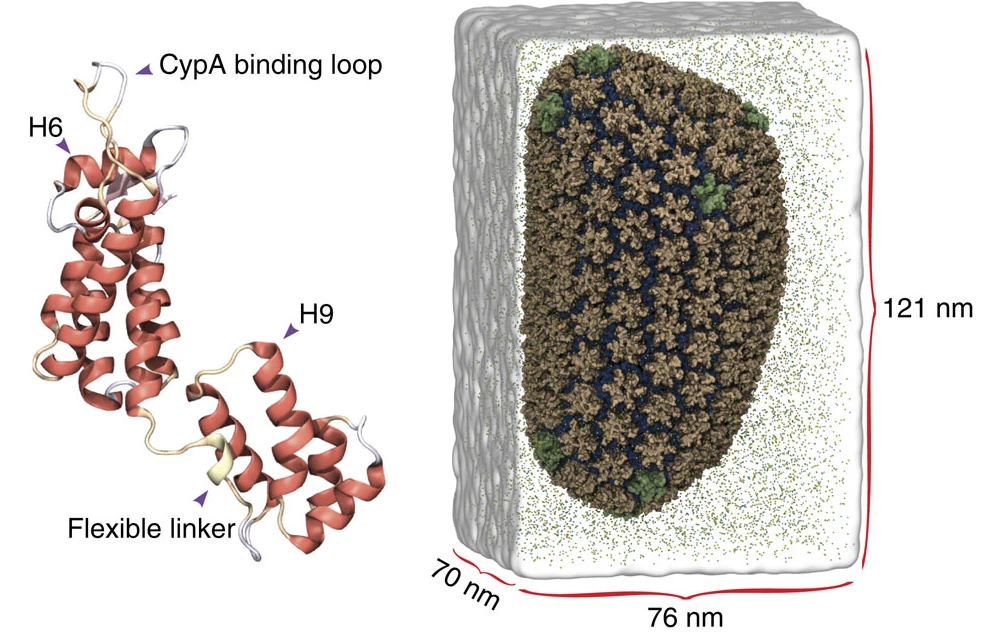
\includegraphics[width=1\columnwidth, trim={0cm 0 0cm 0cm}]{figures/Intro/HIV-1.png}
            \caption{Molecular dynamics simulations of the HIV-1 capsid. Perilla et al.~\cite{Perilla2017} used a simulation containing 64,423,983 atoms to investigate different properties of the HIV-1 capsid at an atomic resolution.}
            \label{fig:hiv_capsid}
      \end{figure}

      \begin{figure}[H]
            \centering
            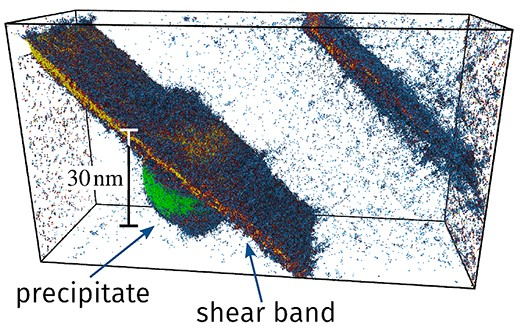
\includegraphics[width=0.9\columnwidth,trim={0cm 0 0cm 0cm}]{figures/Intro/metallic-glass-crack.jpg}
            \caption{Molecular dynamics simulations of shear band formation around a precipitate in metallic glass, as demonstrated by Brink et al.~\cite{Brink2016}.}
            \label{fig:md_simulation_loop}
      \end{figure}
\end{multicols*}

\subsection{Quantum Mechanics and the Schrödinger Equation}

Our current knowledge of physics suggests that the behavior of atoms and molecules is governed by the laws of quantum mechanics, where particles are described by wave functions and probabilities evolving. The physicist Erwin Schrödinger first formulated a mathematical model describing this phenomenon in 1926, which has gotten widespread acceptance and is now known widely as the Schrödinger equation. The Schrödinger equation is a partial differential equation describing how a physical system's wave function evolves over time. It is typically written as:

\begin{equation}
      i \hbar \frac{\partial \Psi}{\partial t} = \hat{H} \Psi
\end{equation}

Where $\Psi$ is the system's wave function, $\hat{H}$ is the Hamiltonian operator describing the system's energy, $t$ is the time, and $\hbar$ is the reduced Planck constant.

The Schrödinger equation provides a way to calculate the future states of a quantum system given the current state of the system. However, solving the Schrödinger equation for systems with many particles is computationally very expensive and quickly becomes infeasible for systems with more than a few particles~\cite{Leimkuhler2015}. Simulating a single water molecule consisting of three nuclei and 10 electrons would require solving a partial differential equation with 39 variables (The molecule consists of two hydrogen atoms, one oxygen atom, and 10 electrons. Each of those 13 objects is described by three spatial coordinates). Consequently, the resulting Shcrödinger equation also includes all 39 variables and looks like this:

\begin{equation}
      i \hbar \frac{\partial \Psi}{\partial t} = -\hbar^2 \sum_{i=1}^{13} \frac{1}{2m_i} \left( \frac{\partial^2 \Psi}{\partial x_i^2} + \frac{\partial^2 \Psi}{\partial y_i^2} + \frac{\partial^2 \Psi}{\partial z_i^2} \right) + U_p (x_1, y_1, z_1, \ldots, x_{13}, y_{13}, z_{13}) \Psi
\end{equation}

Where $m_i$ is the mass of the $i$-th object, $x_i$, $y_i$, and $z_i$ are the spatial coordinates of the $i$-th object, and $U_p$ is the potential energy function of the system.

As the Schrödinger equation is a partial differential equation, it is computationally expensive to solve for systems with many particles, as one quickly runs into the curse of dimensionality.

The Born-Oppenheimer approximation simplifies this problem by exploiting the significant mass difference between electrons and nuclei. From the perspective of fast-moving electrons, the much heavier nuclei appear nearly stationary, which justifies the separation of electronic and nuclear motions, treating the nuclei as classical particles. The electronic degrees of freedom can then be integrated out, deriving a new energy function $U$ that depends solely on nuclear positions.
This potential energy surface $U$ is typically obtained through quantum mechanical calculations or fitted to empirical data.

However, this approach is still just an approximation, and depending on the chosen potential energy function U, the Born-Oppenheimer approximation may neglect certain quantum mechanical effects, causing inaccuracies in the simulation results.


Despite these limitations, the Born-Oppenheimer approximation is widely used in molecular dynamics simulations as it allows for the simulation of systems with many particles in the first place.

After applying the Born-Oppenheimer approximation and using Newton's second law of motion, the Schrödinger equation can be transformed into a system of ordinary differential equations. Each of those equations describes the motion of a single particle and is given by:

\begin{align}
      m_i \frac{d^2 x_i}{dt^2} & = -\frac{\partial U}{\partial x_i} \\
      m_i \frac{d^2 y_i}{dt^2} & = -\frac{\partial U}{\partial y_i} \\
      m_i \frac{d^2 z_i}{dt^2} & = -\frac{\partial U}{\partial z_i}
\end{align}

Where $m_i$ is the mass of the $i$-th particle, $x_i$, $y_i$, and $z_i$ are the spatial coordinates of the $i$-th particle, and $U$ is the newly derived potential energy function of the system.

\subsection{Numerical Integration}

Since the simulation domain potentially consists of a vast number of particles all interacting with each other, it is generally not possible to solve the equations of motion analytically. This problem is known under the N-body problem, and it can be shown that there are no general solutions for systems with more than two particles. We can, however, solve the equations of motion numerically using numerical integration methods. A standard method to solve the equations of motion numerically is the Verlet algorithm. This integration scheme is derived from the Taylor expansion of the position of the $i$-th object $\vec{r}_i$ at time $t - \Delta t$ and $t + \Delta t$ and is given by:

\begin{equation}
      \vec{r}_i(t + \Delta t) = 2 \vec{r}_i(t) - \vec{r}_i(t - \Delta t) + \vec{a}_i(t) \Delta t^2
\end{equation}

Where $\vec{a}_i(t)$ is the acceleration of the $i$-th object at time $t$ and can be calculated from the particle mass and the acting forces using Newton's second law of motion $\vec{a}_i(t) =\frac{F_i}{m_i}= \frac{-\nabla_i U}{m_i}$.

\subsection{Potential Energy Function}

As stated above, the potential energy function $U$ is a critical component of the molecular dynamics simulation as it fundamentally defines the properties of the system. MD simulations use many different potential energy functions, all of which are tailored to describe specific aspects of the system. Those potentials typically use a mixture of 2-body, 3-body, and 4-body interactions between the particles. The 2-body interactions express the effect of Pauli repulsion, atomic bonds, and coulomb interactions, while higher-order interactions allow for potentially asymmetric wave functions~\cite{Leimkuhler2015}.

A common choice for the potential energy function is the Lennard-Jones potential. The simplicity of the Lennard-Jones potential makes it a popular choice for many systems, as it can be computed efficiently and still captures the attractive and repulsive forces between particles quite well. The Lennard-Jones potential is given by:

\begin{equation}
      U_{LJ}(r) = 4 \epsilon \left[ \left( \frac{\sigma}{r} \right)^{12} - \left( \frac{\sigma}{r} \right)^6 \right]
\end{equation}


Where $r$ is the distance between the particles, $\epsilon$ is the depth of the potential well, and $\sigma$ is the distance at which the potential is zero.

\subsection{Simulation Loop}

Using the methods described above, it is possible to simulate the behavior of a system of particles over time. The general simulation loop for a molecular dynamics simulation can be described as follows:

\begin{enumerate}
      \item \textbf{Initialization} \\
            The simulation starts by initializing the positions and velocities of the particles. The initial positions and velocities can be chosen randomly or based on experimental data.

      \item \textbf{Position Updates} \\
            In this step, the positions of the particles are updated using a numerical integration scheme such as the Verlet algorithm.

      \item \textbf{Force Calculation} \\
            The forces acting on the particles are calculated based on the current positions of the particles and the chosen potential energy function $U$.

      \item \textbf{Update Velocities and Accelerations} \\
            The acceleration of each particle is calculated using Newton's second law of motion. The velocities of the particles are then updated using the acceleration and the time step $\Delta t$.

      \item \textbf{Apply External Forces or Constraints} \\
            In this step, the simulation can be modified by applying external forces or constraints to the particles. In this stage, it is possible to introduce boundary conditions, temperature control, or other outside effects to the simulation.

      \item \textbf{Update Time and Repeat} \\
            The simulation time is updated by advancing it by the time step $\Delta t$. The simulation loop returns to step 2 and repeats until the desired number of integration steps is reached.
\end{enumerate}


Many different software packages exist to perform such simulations. Some widely used examples of such systems are LAAMPS\footnote{\url{https://lammps.sandia.gov/}} and GROMACS\footnote{\url{https://www.gromacs.org/}}. Both efficiently solve the underlying N-body problem and provide the user with a high-level interface to specify the simulation parameters.

Many different approaches exist to efficiently solve the N-body problem, and no single best approach works well for all systems as the optimal implementation heavily depends on the simulation state and the hardware's capabilities to perform the simulation. However, LAAMPS and GROMACS use a single implementation and cannot adapt their algorithms to the current simulation state.

In the following section, we will introduce AutoPas, a library designed to efficiently deal with changing simulation states and capable of automatically adapting to the current simulation state to achieve optimal performance.

\section{AutoPas}

AutoPas is an open-source library designed to achieve optimal performance at the node level for short-range particle simulations. On a high level, AutoPas can be seen as a black box performing arbitrary N-body simulations with short-range particle interactions. The main goal of AutoPas is to provide a high-level interface for the user to perform simulations without worrying about the low-level details of the simulation. This is achieved by providing a high-level interface for the user to interact with the library while the library itself takes care of the low-level details of the force calculations

AutoPas provides many different algorithmic implementations for the problem of N-body simulations, each with different performance and memory usage trade-offs. No single implementation is optimal for all simulation scenarios \todo{find reference}, as the optimal implementation depends on the current simulation state.
AutoPas is designed to be adaptive and can periodically switch between different implementations to achieve the best performance for the current simulation state. This is achieved by allowing AutoPas to automatically tune its internal parameters to find the best implementation for the current simulation state.


Since AutoPas provides a high-level interface for short-range N-body simulations, the user specifies the acting forces between the particles and controls the simulation loop. Fortunately, AutoPas also provides \texttt{\gls{mdflexible}}, an example of a typical molecular dynamics simulation implementation.

\subsection{Autotuning in AutoPas}

AutoPas internally alternates between two phases of operation. The first phase is the \emph{tuning phase}, where AutoPas tries to find the best configuration of parameters about a chosen performance metric. This optimal configuration is then used in the following \emph{simulation phase}, assuming that the optimal configuration found in the tuning phase still performs reasonably well during the consequent simulation phase. As the simulation progresses and the characteristics of the system change, the previously chosen configuration can drift arbitrarily far from the actual optimal configuration. To counteract this, AutoPas periodically alternates between tuning and simulation phases to ensure that the used configuration is reasonably close to the optimal configuration.
AutoPas acts as a black box during the simulation phase, solving the force calculations for the underlying N-body problem.


The power of AutoPas comes from its vast amount of tunable parameters and enormous search space. As mentioned, their design limits other software packages like LAAMPS and GROMACS to just one implementation. They can, therefore, operate outside of the theoretical
optimal performance regime. In the following section, we will discuss the tunable parameters in AutoPas and the different tuning strategies available to find the best configuration of parameters for the current simulation state.


\subsection*{Tunable Parameters}

AutoPas currently provides six tunable parameters, which can mostly\footnote{There are some exceptions as some choices of parameters are incompatible with each other.} be combined freely. A collection of parameters is called a \emph{Configuration}, and the set of all possible configurations is called the \emph{Search Space}. A configuration consists of the following parameters:

\begin{enumerate}[label=\textbf{\arabic*.}]
      \item \textbf{Container Options:} \\
            The container options are related to the data structure used to store the particles. The most important categories of data structures in this section are:
            \begin{enumerate}
                  \item \textbf{DirectSum} \\
                        DirectSum does not use any additional data structures to store the particles. Instead, it simply holds a list of all particles and performs a brute-force calculation of the forces between all pairs of particles. This results in a complexity of $O(N^2)$ distance checks in each iteration. This method is simple and does not require additional data structures, but it has an inferior complexity, making it unsuitable for larger simulations. \textit{Generally should not be used except for tiny systems or demonstration purposes.~\cite{VICCIONE2008625}}
                  \item \textbf{LinkedCells} \\
                        LinkedCells segments the domain into a regular cell grid and only considers interactions between particles from neighboring cells. This results in the trade-off that particles further away than the cutoff radius are not considered for the force calculation. This is not a big issue in practice, as all short-range forces drop off quickly with distance anyway. Additionally, LinkedCells provides a high cache hit rate as particles inside the same cell can be stored contiguously in memory. Typically, the cell size is chosen to be equal to the cutoff radius $r_c$, meaning that each particle only needs to check the forces with particles inside the $3\times3\times3$ cell grid around it as all other particles are guaranteed to be further away than the cutoff radius. This reduction in possible interactions can result in a complexity of just $O(N)$ distance checks in each iteration. However, there is still room for improvement as constant factors can be pretty high. This is especially obvious, as most distance checks performed by LinkedCells still do not contribute to the force calculation~\cite{GRATL2019748}. This trend can be explained due to the uneven scaling of sphere and cube volumes, especially for higher dimensions. For example, in 3D, the ratio of the volume of a sphere with radius $r_c$ to the volume of a cube with side length $3r_c$ is given by:

                        \begin{equation}
                              \frac{\text{Interaction Volume}}{\text{Search Volume}} =
                              \frac{V_{sphere}(r_c)}{V_{cube}(3r_c)} = \frac{\frac{4}{3}\pi r_c^3}{(3r_c)^3} = \frac{4}{81}\pi \approx 0.155
                        \end{equation}

                        This means that only about 15.5\% of all particles present in the $3\times3\times3$ cell grid around a particle are within the cutoff radius.

                        \textit{However, still generally good for large, homogeneous\footnote{Homogeneous in this context, the particles are distributed evenly across the domain.} systems.}

                  \item \textbf{VerletLists} \\
                        VerletLists is another approach to creating neighbor lists for the particles. Contrary to LinkedCells, VerletLists does not rely on a regular grid but instead uses a spherical region around each particle to determine its relevant neighbors.
                        The algorithm creates and maintains a list of all particles present in a sphere within radius $r_c \cdot s$ around each particle, where $r_c$ is the cutoff radius and $s>1$ is the skin factor allowing for a buffer zone around the cutoff radius.
                        By choosing a suitable buffer zone, such that no fast-moving particle can enter the cutoff radius unnoticed, it is possible to only recalculate the neighbor list every few iterations. This approach can benefit systems with high particle density and frequent interactions, as the neighbor list only needs to be updated every $n$ iteration. This results in a complexity of $O(N)$ distance checks in each iteration.
                        We can repeate the calculation from above to determine the ratio of the interaction volume to the search volume for VerletLists:

                        \begin{equation}
                              \frac{\text{Interaction Volume}}{\text{Search Volume}} =
                              \frac{V_{sphere}(r_c)}{V_{sphere}(r_c \cdot s)} = \frac{\frac{4}{3}\pi r_c^3}{\frac{4}{3}\pi (r_c \cdot s)^3} = \frac{1}{s^3}
                        \end{equation}

                        The ratio can be adjusted by changing the skin factor $s$ this time.         Ideally, the skin factor should be chosen so the ratio is close to 1. However, this reduces the buffer zone around the cutoff radius, meaning that the neighbor list needs to be updated more frequently. We conclude that choosing a skin factor that is too small can result in particles entering the cutoff radius unnoticed, leading to incorrect results, while choosing a skin factor that is too large can result in unnecessary distance checks.

                        Compared to LinkedCells, VerletLists can be constructed so that there are few unnecessary distance checks. However, constructing the neighbor list is quite memory intensive and can result in a high memory overhead. Additionally, the neighbor list needs to be updated every few iterations, which can result in a performance overhead.

                        \textit{Generally good for large systems with high particle density.}

                  \item \textbf{VerletClusterLists} \\
                        VerletClusterLists differ from regular VerletLists in the way the neighbor lists are stored. Instead of storing the neighbor list for each particle separately, $n_{cluster}$ particles are grouped into a so-called \emph{cluster}, and a single neighbor list is created for each cluster. This reduces memory overhead as the neighbor list only needs to be stored once for each cluster. Whenever two clusters are close, all interactions between the particles in the two clusters are calculated. This also results in a complexity of $O(N)$ distance checks in each iteration.

                        The main advantage of VerletClusterLists is the reduced memory overhead compared to regular VerletLists. However, constructing the neighbor list is still quite memory intensive and can result in a high memory overhead.

                        \textit{Generally suitable for large systems with high particle density}

            \end{enumerate}

      \item \textbf{Load Estimator Options:} \\
            The Load Estimator Options are related to the way the simulation is parallelized. The load estimator is responsible for estimating the computational load of each MPI rank and how the work is distributed among the ranks. In this thesis, however, we will not further detail the Load Estimator Options as we primarily focus on the tuning aspect of single-node simulations.

      \item \textbf{Traversal Options:} \\
            These options are related to the traversal algorithm used to calculate the forces between the particles. The traversal determines the order in which the particles are visited and how the forces are calculated.
            The different traversal options efficiently prevent race conditions when using multiple threads and allow load balancing at the node level ~\cite{SECKLER2021101296}.

            Many different traversal algorithms are available in AutoPas, each with different performance and optimization potential trade-offs. In the following, we will discuss the most interesting traversal categories:

            \begin{enumerate}

                  \item \textbf{Colored Traversal} \\
                        Since both LinkedCells and VerletLists only consider interactions with particles from neighboring cells/particles, it is possible to parallelize the force calculation by calculating forces for particles in different cells in parallel. This is, however, only possible if all simultaneously calculated particles do not share familiar neighbors, as this would introduce data races when updating the forces of the particles. This is where the concept of coloring comes into play. Coloring is a way to assign a color to each cell so that cells with the same color do not share familiar neighbors. This allows for the force calculation of particles in cells with the same color to be parallelized trivially, as data races are impossible.

                        There are many different ways to color the domain. Some of the most interesting coloring options are:
                        \begin{itemize}
                              \item \textbf{C01} \\
                                    The C01 traversal is the simplest way of coloring the domain, as all cells get colored the same way. This means all cells can be perfectly parallelized (embarrassingly parallel) as long as Newton 3 is disabled. This, however, also means that all forces are calculated twice, once for each of the two particles involved.

                              \item \textbf{C18} \\
                                    The C18 traversal is a more sophisticated way of coloring the domain. The domain is divided into 18 colors, so no two neighboring cells share the same color. This method also utilizes the Newton 3 law to reduce the number of force calculations. This is achieved by only computing the forces with forward neighbors (neighbors with greater index.) ~\cite{GRATL2022108262}

                        \end{itemize}

                  \item \textbf{Sliced Traversal} \\
                        Sliced Traversal is a way to parallelize the force calculation by dividing the domain into different slices and calculating the forces for particles in different slices in parallel. It uses locks to prevent data races ~\cite{GRATL2022108262}.

            \end{enumerate}


      \item \textbf{Data Layout Options:} \\
            The Data Layout Options determine how the particles are stored in memory. The two possible data layouts are:
            \begin{enumerate}
                  \item \textbf{SoA} \\
                        The SoA (Structure of Arrays) data layout stores the particles' properties in separate arrays. For example, all particles' x-,y- and z-coordinates are stored in separate arrays. This data layout is beneficial for vectorization as the properties of the particles are stored contiguously in memory. This allows for efficient vectorization of the force calculations as the properties of the particles can be loaded into vector registers in a single instruction. \todo{find reference}

                  \item \textbf{AoS} \\
                        The AoS (Array of Structures) data layout stores all particle properties in many structures. This allows for efficient cache utilization as the properties of the same particle are close to each other in memory. However, this data layout is not beneficial for vectorization as the properties of the particles are not stored contiguously in memory. This means that the properties of the particles need to be loaded into vector registers one by one, which can result in inefficient vectorization of the force calculations. \todo{find reference}
            \end{enumerate}



      \item \textbf{Newton 3 Options:} \\
            The Newton 3 Options relate to how the forces between the particles are calculated. The Newton 3 law states that for every action, there is an equal and opposite reaction \todo{cite}. This means that the force between two particles is the same, regardless of which particle is the source and which is the target. In Molecular Dynamics simulations, this rule can be exploited to reduce the distance checks needed to calculate the forces between all pairs of particles by a factor of 2. The two possible Newton 3 options are:
            \begin{enumerate}
                  \item \textbf{Newton3 Off} \\
                        If Newton 3 is turned off, the forces between all pairs of particles are calculated twice, once for each particle. This results in a constant overhead of factor 2.

                  \item \textbf{Newton3 On} \\
                        If Newton 3 is turned on, the forces between all pairs of particles are calculated only once. There is no more overhead due to recalculating the forces twice, but turning on Newton 3 requires additional bookkeeping, especially in multi-threaded environments. This results in more complicated traversal algorithms and can result in a performance overhead.
                        \textit{Generally should be turned on whenever available.}
            \end{enumerate}

      \item \textbf{Cell Size Factor:} \\
            The Cell Size Factor is a parameter that is used to determine the size of the cells in the LinkedCells-Container\footnote{The option is also relevant for other containers such as VerletLists those configurations internally also build their neighbor lists using a Cell Grid }. The cell size factor is typically chosen to be equal to the cutoff radius $r_c$, meaning that each particle only needs to check the forces with particles inside the $3\times3\times3$ cell grid around it as all other particles are guaranteed to be further away than the cutoff radius. We saw in the previous section that this could result in a high number of unnecessary distance checks as only about 15.5\% of all particles present in the $3\times3\times3$ cell grid around a particle are within the cutoff radius. By choosing smaller cell sizes, this ratio can be increased, reducing the number of unnecessary distance checks. However, the increased overhead of managing more cells quickly offset the performance gain.

\end{enumerate}

\subsection*{Tuning Strategies}

Tuning strategies are the heart of AutoPas. They implement the critical functionality of AutoPas' dynamic tuning aspect. The main goal of the tuning strategies is to find the best parameters for the current simulation state, which can then be used for the following simulation phase.

The default tuning strategy in AutoPas uses a brute-force approach to find the best parameters for the current simulation state by trying out all possible combinations of parameters and choosing the one that optimizes the chosen performance metric (e.g., time, energy usage). This approach is called \emph{Full Search} and is guaranteed to find the best parameters for the current simulation state. However, it is typically very costly in terms of time and resources as it has to spend a lot of time measuring bad parameter combinations. This is a big issue as the number of possible parameter combinations can grow exponentially with the number of parameters. This makes the full search approach infeasible, especially if more tunable parameters are added to AutoPas.

To overcome this issue, AutoPas provides a couple of different tuning strategies that can be used to reduce the number of parameter combinations that need to be tested. This is generally achieved by allowing the tuning strategy to modify the set of parameters that need to be tested, thereby reducing the total number of configurations that need to be tested. It is, therefore, of great interest to develop tuning strategies that can effectively prune the search space, as this can result in a significant speedup of the tuning process.

In the following, we will briefly discuss the basic tuning strategies available in AutoPas:

\begin{enumerate}
      \item \textbf{Full Search} \\
            The Full Search strategy is the default tuning strategy in AutoPas. It tries out all possible combinations of parameters and chooses the one that optimizes the chosen performance metric. It is guaranteed to find the best parameters for the current simulation state, but as mentioned before, it is very costly.

      \item \textbf{Random Search} \\
            The Random Search strategy is a simple tuning strategy that randomly samples a given number of configurations from the search space and chooses the one that optimizes the chosen performance metric. This approach is faster than the Full Search strategy as it does not need to test all possible combinations of parameters. However, it is not guaranteed that the best parameters for the current simulation state will be found, which could suggest a wrong configuration.

      \item \textbf{Predictive Tuning} \\
            The Predictive Tuning strategy attempts to extrapolate previous measurements to predict how the configuration would perform in the current simulation state. It prunes the search space only, keeping configurations predicted to perform reasonably well. The extrapolations are accomplished using methods such as linear regression or constructing polynomial functions through the data points. The method generally works well but is very sensitive to timing fluctuations.

      \item \textbf{Bayesian Search} \\
            Two implementations of Bayesian tuning exist in AutoPas. Those methods apply Bayesian optimization techniques to predict suitable configurations using performance evidence from previous measurements.

      \item \textbf{Rule Based Tuning} \\
            The Rule Based Tuning strategy uses a set of predefined rules to automatically filter out configurations that will perform poorly. The rules are built up using the configuration order of the form:
            \begin{small}
                  \begin{verbatim}
            if numParticles < lowNumParticlesThreshold:
                  [dataLayout="AoS"] >= [dataLayout="SoA"] with same 
                        container, newton3, traversal, loadEstimator;
            endif
            \end{verbatim}
            \end{small}
            The data layout "AoS" is generally better than "SoA" if the number of particles is below a certain threshold. The rule-based method can be very effective as expert knowledge can be encoded into the rules. Unfortunately, it is also its biggest drawback, as creating a good set of rules is not trivial.
\end{enumerate}


This thesis aims to extend these tuning strategies with a new approach based on Fuzzy Logic. Conceptually, this new fuzzy logic-based tuning strategy is very similar to the rule-based tuning strategy as it uses expert knowledge of fuzzy rules to prune the search space. However, contrary to classical rules, fuzzy logic can deal with imprecise and uncertain information, which allows it to only partially activate rules and assign a degree of activation to each rule. All the rules can then be combined based on their degree of activation rather than just following the binary true/false logic. This allows for a more nuanced approach and allows the tuning strategy to interpolate the effect of many different rules to choose the best possible configuration, even if there is no direct rule for this specific case.

Such fuzzy logic-based approaches can be especially beneficial when dealing with complex systems \todo{cite} as they allow for a more nuanced approach to the problem. In the following section, we will introduce the basic concepts of fuzzy logic and how it is used to create a new tuning strategy for AutoPas.


\section{Fuzzy Logic}

Fuzzy Logic is a mathematical framework that allows for reasoning under uncertainty. It is an extension of classical logic and extends the concept of binary truth values (false/0 and true/ 1) to a continuous range of truth values in the interval $[0, 1]$. This allows for a more nuanced representation of the truth values of statements, which can be beneficial when dealing with imprecise or uncertain information. Instead of just having true or false statements, it is now possible for statements to be, for example, 40\% true.

This concept is beneficial when modeling human language, as the words tend to be imprecise. For example, "hot" can mean different things to different people. For some people, a temperature of 30 degrees Celsius might be considered hot, while for others, a temperature of 40 degrees Celsius might be considered hot. There is no clear boundary between what is considered hot and what is not, but rather a gradual transition between the two. Fuzzy Logic allows for modeling such gradual transitions by assigning a degree of truth to each statement.

\todo{make image}


\subsection{Fuzzy Sets}

Mathematically, the concept of Fuzzy Logic is based on Fuzzy Sets. A Fuzzy Set is a generalization of a classical set where an element can lie somewhere between being a set member and not being a member. Instead of having a binary membership function that assigns a value of 1 to elements that are members of the set and 0 to elements that are not, elements in a fuzzy set have a certain degree of membership in the set. This degree of membership is a value in the interval $[0, 1]$ that represents the degree to which the element is a member of the set, with 0 meaning that the element is not a member of the set at all and one meaning that the element is a full member of the set.


Formally a fuzzy set $\tilde{A}$ over a crisp/standard set $X$ is defined by a membership function
\begin{equation}
      \mu_{\tilde{A}}: X \rightarrow [0, 1]
\end{equation}
that assigns each element $x \in X$ a value in the interval $[0, 1]$ that represents the degree to which $x$ is a member of the set $\tilde{A}$. The classical counterpart is classically written using the element operator $\in_A: X \rightarrow \{true, false\}$.

The shape of the function can be chosen freely and depend on the specific application, but typical choices involve triangular, gaussian, or sigmoid-shaped functions.

\todo{insert image}


\subsection{Fuzzy Logic Operations}

Fuzzy Sets are a generalization of classical sets, and as such, they also support the classical set operations of union, intersection, and complement. However, how these operations are defined differs from the classical case, as the membership functions are continuous and can take on any value in the interval $[0, 1]$.

The extension of classical sets makes use of the so-called De Morgan Triplets. Such a triplet $(\top, \bot, \neg)$ consists of a t-norm $\top : [0, 1] \times [0, 1] \rightarrow [0, 1]$, a t-conorm $\bot : [0, 1] \times [0, 1] \rightarrow [0, 1]$ and a strong complement operator $\neg : [0, 1] \rightarrow [0, 1]$. Those operators generalize the classical logical operators, which are only defined on the binary truth values $\{0, 1\}$ to values from the continuous interval $[0, 1]$. $\top$ can generalize the logical AND operator to fuzzy sets, while $\bot$  and $\neg$ can generalize the logical OR and NOT operators. The binary operators $\top$ and $\bot$ are often written in infix notation as $a \; \top \; b$ and $a \; \bot \; b$, similar to how classical logical operators are written.


For the t-norm $\top$ to be valid, it needs to satisfy the following properties:

\begin{align*}
      a \; \top \; b                & = b \; \top \; a                                              & \quad \text{//Commutativity}    \\
      a \; \bot \; b                & \leq c \; \top \; d  \quad \text{if }  a\leq b \land b \leq d & \quad \text{//Monotonicity}     \\
      a \; \top \; (b \; \top \; c) & = (a \; \top \; b) \; \top \; c                               & \quad \text{//Associativity}    \\
      a \; \top \; 1                & = a                                                           & \quad \text{//Identity Element}
\end{align*}

\todo{fix the layout}

The complement operator $\neg$ needs to satisfy the following properties:

\begin{align*}
      \neg 0             & = 1                       & \quad \text{//Boundary Conditions} \\
      \neg 1             & = 0                       & \quad \text{//Boundary Conditions} \\
      \neg y \leq \neg x & \quad \text{if } x \leq y & \quad \text{//Monotonicity}
\end{align*}

Additionally, it is called a strong complement operator if it satisfies the following property:

\begin{align}
      \neg \neg x = x & \quad \text{//Involution}                                       \\
      \neg y < \neg x & \quad \text{if } x < y    & \quad \text{ //Strong Monotonicity}
\end{align}


The standard negation operator $\neg x = 1 - x$ is a strong complement operator as it satisfies all the properties above and is the most common choice for the negation operator in practice.

Some common choices for t-norms and t-conorms used in practice are shown in Table~\ref{tab:tnorms}.

\begin{table}[H]
      \centering
      {\renewcommand{\arraystretch}{1.2}
            \begin{tabular}{|c|c|c|c|}
                  \hline
                  T-Norm Name & T-Norm   $a \top b$                                                                              & Corresponding T-Conorm      $a \bot b$                                                           \\
                  \hline
                  Minimum     & $\min(a, b)$                                                                                     & $\max(a, b)$                                                                                     \\
                  Product     & $a \cdot b$                                                                                      & $a + b - a \cdot b$                                                                              \\
                  Lukasiewicz & $\max(0, a + b - 1)$                                                                             & $\min(1, a + b)$                                                                                 \\
                  Drastic     & $\begin{cases} b & \text{if } a = 1 \\ a & \text{if } b = 1 \\ 0 & \text{otherwise} \end{cases}$ & $\begin{cases} b & \text{if } a = 0 \\ a & \text{if } b = 0 \\ 1 & \text{otherwise} \end{cases}$ \\
                  Einstein    & $\frac{a \cdot b}{2 - (a + b - a \cdot b)}$                                                      & $\frac{a + b}{1 + a \cdot b}$                                                                    \\

                  \hline
            \end{tabular}
      }
      \caption{Common T-Norms and corresponding T-Conorms concerning the standard negation operator $\neg x = 1 - x$
            for $a, b \in [0, 1]$}
      \label{tab:tnorms}
\end{table}

In the following sections, we will only consider the standard negation operator, the minimum t-norm, and the maximum t-conorm, as they are the most common choices in practice in fuzzy logic systems. However, if needed, the exact choices can be easily exchanged for other t-norms and t-conorms.


With these choices of t-norms, t-conorms, and negation operators, it is possible to define the classical set operations of union, intersection, and complement for fuzzy sets. The operations are defined as follows:


\begin{itemize}

      \item \textbf{Intersection} \\
            The intersection $\tilde{C} = \tilde{A} \cap \tilde{B}$ of two fuzzy sets $\tilde{A}$ and $\tilde{B}$ both defined over the same crisp set $X$ is defined by the new membership function
            \begin{equation}
                  \mu_{\tilde{C}}(x) = \min(\mu_{\tilde{A}}(x), \mu_{\tilde{B}}(x))
            \end{equation}
            This means that the degree of membership of an element $x$ in the intersection set $\tilde{C}$ is just the minimum of the degrees of membership of $x$ in the sets $\tilde{A}$ and $\tilde{B}$.
      \item \textbf{Union} \\
            The union $\tilde{C} = \tilde{A} \cup \tilde{B}$ of two fuzzy sets $\tilde{A}$ and $\tilde{B}$ both defined over the same crisp set $X$ is defined by the new membership function
            \begin{equation}
                  \mu_{\tilde{C}}(x) = \max(\mu_{\tilde{A}}(x), \mu_{\tilde{B}}(x))
            \end{equation}
            This means that the degree of membership of an element $x$ in the union set $\tilde{C}$ is just the maximum of the degrees of membership of $x$ in the sets $\tilde{A}$ and $\tilde{B}$.

      \item \textbf{Complement} \\
            The complement $\tilde{C} = \neg \tilde{A}$ of a fuzzy set $\tilde{A}$ defined over the crisp set $X$ is defined by the standard negation operator
            \begin{equation}
                  \mu_{\tilde{C}}(x) = 1 - \mu_{\tilde{A}}(x)
            \end{equation}
            Again, this means that the degree of membership of an element $x$ in the complement set $\tilde{C}$ is just $1$ minus the degree of membership of $x$ in the set $\tilde{A}$.
\end{itemize}

\todo{add grafical representation of the operations}

\subsection{Linguistic Variables}

Linguistic variables collect multiple fuzzy sets defined over the same crisp set $X$ into a single object. This variable then allows us to reason about the possible states of the variable more naturally.

For example, the linguistic variable "temperature" might have the linguistic terms \emph{cold} \emph{warm}, and \emph{hot}, each of which is defined by a fuzzy set. This representation is very natural as it abstracts away the specific temperature values and allows us to reason about the temperature in a more human-like way.

All the underlying fuzzy sets can be chosen arbitrarily and can also overlap with each other.

\todo{add grafical representation of the linguistic variable}

\subsection{Fuzzy Logic Rules}

Fuzzy Logic Rules are a way to encode expert knowledge into a Fuzzy Logic system. The rules specify the relationship between input and output variables of the system and, therefore, are the backbone of fuzzy logic systems.
The rules are typically encoded in a human-readable way and often have the form "$\text{IF} \; \text{antecedent} \; \text{THEN} \; \text{consequent}$" where both the antecedent and the consequent are fuzzy sets. The antecedent is a condition that must be satisfied for the rule to be applied, while the consequent is the action taken if the rule is applied. Since we are not dealing with binary truth values, the antecedent can only be partially satisfied, and consequently, the rule is only partially applied.

The antecedent can be arbitrarily complicated and involve multiple fuzzy sets and logical operators. The consequent is typically a single fuzzy set modified by the rule but could theoretically be arbitrarily complicated. In this work, we allow rules following the grammar defined below:

%makro for fuzzy set
\newcommand{\fuzzyset}{\langle \text{fuzzy set} \rangle}

\newcommand{\fuzzyrule}{\langle \text{rule} \rangle}


\begin{align*}
      \fuzzyrule  ::= & \ \ \text{IF} \ \fuzzyset \ \text{THEN} \ \fuzzyset & \text { //Rule}        \\[10pt]
      \fuzzyset  ::=  & \ \ (\; \fuzzyset \;)                               & \text { //Parentheses} \\
                      & |  \ \fuzzyset \ \text{AND}  \ \fuzzyset            & \text { //Conjunction} \\
                      & |  \ \fuzzyset \ \text{OR} \  \fuzzyset             & \text { //Disjunction} \\
                      & |  \ \text{NOT} \ \fuzzyset                         & \text { //Negation}    \\
                      & |  \ \tilde{A} \ =\ a                               & \text { //Selection}   \\
\end{align*}

The boolean operators AND, OR, and NOT represent the set operations of intersection, union, and complement, respectively.


Using this grammar, a typical rule might look like this:

\begin{equation}
      \text{IF} \;( \tilde{A} = a \; \text{AND} \; \tilde{B} = b )\; \text{THEN} \; \tilde{C} = c
\end{equation}

This rule states that if the state of the linguistic variable $A$ is $a$ and the state of the linguistic variable $B$ is $b$, then the state of the linguistic variable $C$ should be $c$. However, contrary to classical logic, the rule does not have to activate fully but can have a degree of activation in the interval $[0, 1]$. Should the antecedent be only partially true (for example, if $\mu_{\tilde{A}}(a) = 0.8$ and $\mu_{\tilde{B}}(b) = 0.6$), the rule is only partially applied and the effect of adapting the consequent is reduced accordingly? In the example above, the degree of activation of the rule would be $\min(0.8, 0.6) = 0.6$.

The inference step can be seen as an extension of the boolean implication operator

\[\text{IF} \; \text{antecedent} \; \text{THEN} \; \text{consequent} \iff \text{antecedent} \implies \text{consequent}\]

Moreover, it could be deduced from the choice of the t-norm and t-conorm operators and would lead to $(a \implies b) = \neg a \lor b = \max(1-a,b)$. However, the Mamdani implication is typically used as the AND operation $\min(a,b)$. From a logical point of view, this choice is counterintuitive as it violates the standard definition. However, in the context of fuzzy systems, it is a perfect choice for computing the degree of validity for a rule~\cite {BouchonMeunier1995}. In practice, we are not interested in the resulting fuzzy set of the implication but rather in the extent to which the consequent should be adapted. Therefore, we introduce a slightly different inference algorithm:

\vspace{1em}

Consider the rule $\text{IF} \; \tilde{A} = a \; \text{THEN} \; \tilde{C} = c$

\begin{enumerate}
      \item Obtain the input values $(x_1, x_2, \ldots, x_n) \in X_{A}$ occuring in the crisp set of the antecedent.
      \item Evaluate the degree of membership $\mu$ those input values have in the antecedent. This is the degree to which the antecedent is satisfied, and the rule is activated.
      \item Define a new fuzzy set $R=\tilde{C}\uparrow \mu$ where $\uparrow$ is the cut operator.
            This operator is defined as $\mu_{R}(x) = \min(\mu_{\tilde{C}}(x), \mu)$, which means that it cuts off all membership values of the fuzzy set $\tilde{C}$ that are above the degree of activation $\mu$. This resulting set $R$ contains the information to which extent the consequent should be adapted. We see that in the extreme cases where $\mu = 0$, the set $R$ is also empty and does not affect further computations. If $\mu = 1$, the rule is activated fully, and the set $R$ is equal to $\tilde{C}$. In all other cases, the set $R$ is trimmed to the extent of activation.
\end{enumerate}

\subsection{Defuzzification}

The final step in a Fuzzy Logic system is the defuzzification step. In this step, the fuzzy output of the system is converted back into a crisp value that can be used to control natural-world systems. The first step in defuzzification is to collect all the rules operating on the same output variable and combine their trimmed consequents into a single fuzzy set. This is done by just taking the fuzzy union of all those consequences, which results in a new fuzzy set that represents the combined effect of all the rules on the output variable. This fuzzy set can be converted back into a single crisp value representing some aspect of the fuzzy set using a defuzzification method.

There are many different ways to defuzzify a fuzzy set. Some of the most common methods are:

\begin{itemize}
      \item \textbf{Centroid} \\
            The Centroid method calculates the center of mass of the fuzzy set and returns this value as the crisp output. This method is intuitive as it tries to find a weighted interpolation of all the activated fuzzy sets. It is defined as:

            \begin{equation}
                  \text{Centroid} = \frac{\int_X x \cdot \mu_{\tilde{C}}(x) \, dx}{\int_X \mu_{\tilde{C}}(x) \, dx}
            \end{equation}

      \item \textbf{Mean of Maximum} \\
            The Mean of Maximum method calculates all the input values that result in the maximum membership value of the fuzzy set and returns the average of these values as the crisp output. When there is just one maximum value, this method can be thought of as just returning the x-position of the most likely value.

            It is defined as follows:

            \begin{equation}
                  \text{Mean of Maximum} = \frac{\int_{X'} x \, dx}{\int_{X'}  \, dx}
            \end{equation}
            where $X' = \{x \in X \, | \, \mu_{\tilde{C}}(x) = \max(\mu_{\tilde{C}}(x))\}$ is the set of all input values that result in the maximum membership value of the fuzzy set.



      \item \textbf{Weighted Average} \\
            The Weighted Average method calculates the average of all the input values weighted by their membership values. Contrary to the Centroid method, which integrates over the whole domain, the Weighted Average method only considers a singular point from each membership function where the membership value is maximal. This can be seen as a simplification of the Centroid method and is defined as:

            \begin{equation}
                  \text{Weighted Average} = \frac{\sum_{x \in X'} x \cdot \mu_{\tilde{C}}(x)}{\sum_{x \in X'} \mu_{\tilde{C}}(x)}
            \end{equation}
            where $X'$ is the set of all input values resulting in their fuzzy set's maximum membership value.
\end{itemize}

Also, many other methods exist to defuzzify a fuzzy set, but the ones mentioned above are the most common choices in practice. This thesis focuses on the Centroid and the Mean of Maximum methods.


\subsection{Structure of creating a Fuzzy Logic System}

All the building blocks of a Fuzzy Logic System have been introduced in the previous sections and can now be combined to create a complete Fuzzy Logic System. The general structure of a Fuzzy Logic System is as follows:

\begin{enumerate}
      \item \textbf{Fuzzification} \\
            The first step in a Fuzzy Logic System is to convert the crisp input values into fuzzy sets. This is done by evaluating the membership functions of the fuzzy sets at the crisp input values. This results in a bunch of membership values, which can be used to calculate the boolean operations of the antecedents of the rules.

      \item \textbf{Inference} \\
            The next step is to apply the fuzzy logic rules to the fuzzy input values. This is done by using the degree of membership of the input values in the rules' antecedents to calculate each rule's activation degree. The consequent of each rule is then cut by the degree of activation of the rule to determine the effect of the rule on the output variable. This results in many fuzzy sets representing all the active effects on the output variable.

      \item \textbf{Aggregation} \\
            The fuzzy sets resulting from the inference step are combined into a single fuzzy set containing the combined effect of all the rules on the output variable. This is done by taking the fuzzy union of all the fuzzy sets.

      \item \textbf{Defuzzification} \\
            The final step is to convert the fuzzy output value into a crisp value that can be used to control natural-world systems. This is done by applying a defuzzification method to the fuzzy set representing the combined effect of all the rules on the output variable.
\end{enumerate}


If the system is finished, it can be seen as a black box that takes crisp input values and returns crisp output values similar to a function $f: X \rightarrow \mathbb{R}$.


Using such a system, however, requires much expert knowledge as the rules and the membership functions of the fuzzy sets need to be defined by hand. This can be time-consuming and sometimes even impossible if the system is too complex. Luckily, other methods exist that attempt to automate defining the parameters of the fuzzy logic system. Some standard methods are:

\begin{itemize}
      \item \textbf{Genetic Algorithms} \\
            Genetic Algorithms are a class of optimization algorithms that are inspired by the process of natural selection. They maintain a population of candidate solutions to a problem and iteratively improve them by applying genetic operators such as mutation and crossover. Genetic Algorithms can optimize the parameters of a fuzzy logic system by treating the parameters as an individual's genes and the system's performance as the individual's fitness. By iteratively evolving the population of individuals, it is possible to find a set of parameters that optimizes the performance of the fuzzy logic system.

      \item \textbf{Data Driven Methods} \\
            Data Driven Methods are a class of optimization algorithms that work by using data to optimize the parameters of a fuzzy logic system. Those methods are often based on machine learning algorithms such as decision trees. They work by trying to find some interpretable representation of the data that can be used to define concrete rules for the fuzzy logic system.

      \item \textbf{Fuzzy Clustering} \\
            Fuzzy Clustering is a class of clustering algorithms that work by assigning each data point to a cluster with a certain degree of membership. It can be used to optimize the parameters of a fuzzy logic system by treating the data points as the input values of the system and the clusters as the fuzzy sets of the system. By iteratively updating the clusters to better fit the data points, it is possible to find a set of parameters that optimizes the performance of the fuzzy logic system.
            \todo{find sources for all of them}
\end{itemize}